\ProvidesFile{appendices/ap-FastTiming.tex}

\chapter{UTILIZING INDUCED CURRENTS FOR FAST TIMING INFORMATION IN PIXEL DETECTORS TO ACHIEVE FOUR-DIMENSIONAL TRACKING}
\label{Fast_Timing}

\section{Overview and Motivation}
To increase the physics reach potential of high-energy collision experiments, the HL-LHC upgrade aims to vastly increase the instantaneous luminosity of the LHC beyond its current value. 
As instantaneous collider luminosity increases, silicon pixel tracking detectors in HL-LHC experiments are faced with the challenge of resolving the trajectories of high-energy particles in environments with high pileup, rate, and radiation.
With an expected pileup of up to 200 events per bunch crossing at the HL-LHC, with an average distance between vertices \sim$\SI{500}{\micron}$ and timing rms \sim$\SI{150}{\ps}$~\cite{CARTIGLIA201747}, precise timing information would dramatically improve the reconstruction process by providing another dimension to separate vertices and avoid a loss of events due to pileup degradation.

To achieve precise timing measurements for HL-LHC collision, the CMS collaboration has designed the MIP timing sub-detector (MTD) to measure arrival times of high-energy particles~\cite{CMS:2667167}.
The hybrid design of the MTD places LYSO scintillating crystals read-out by silicon photo-multipliers (SiPM) in the barrel, as well as low gain avalanche diodes (LGADs) in the end-caps, between the silicon tracker and ECAL layers, to complement timing information provided by the ECAL and provide time-of-flight information with timing resolutions on the order of a few tens of picoseconds.

Hybrid silicon pixel detectors consisting of silicon sensors bump-bonded to readout chips currently constitute state-of-the-art silicon tracking detector technology and are the front-runners for track reconstruction and vertex identification in the high instantaneous luminosity environment of the HL-LHC.
While these detectors have high granularity for spatial measurements, the timing resolution is relatively poor, because the sensors and readout electronics have cumbersome interconnects with high capacitance additions to the pre-amplifiers. 
Pixel detectors able to provide four-dimensional information for tracking have not yet been realized.

\section{Small Pixels, Signal, and Noise}
Collaborating with FNAL scientist, Dr. Ron Lipton, we explore whether small, low-capacitance pixels integrated with fast electronics show promise for realizing the timing resolution required for four-dimensional tracking.
Smaller pixels provide better resolution, have better efficiency by avoiding in-pixel pileup, and have higher radiation tolerance due to less leakage current per pixel~\cite{Garcia-Sciveres_2018}.

\begin{figure}[htb]
  \begin{center}
    \begin{tabular}{c}
        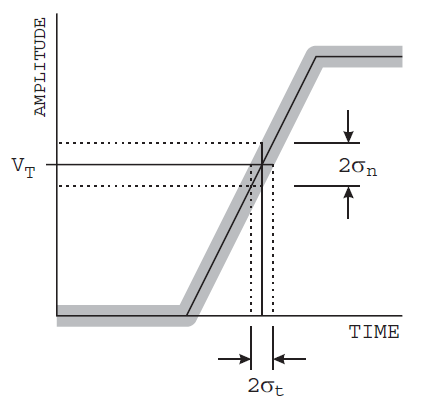
\includegraphics[width=0.45\textwidth]{fig_FastTiming/Jitter.png}
    \end{tabular}
    \caption{Fluctuations in signal amplitude crossing a voltage threshold translate into timing fluctuations called ``jitter.''
            }            
    \label{Jitter}
  \end{center}
\end{figure}
The timing resolution ($\sigma_t$) in a system limited by jitter (i.e. early or late firing fluctuations due to the presence of noise as illustrated in figure~\ref{Jitter}) can be expressed as:
\begin{linenomath*}
\begin{align}
\sigma_t =\frac{\sigma_n}{\frac{d V}{d t}\vert_{V_T}} \approx t_r\frac{Noise}{Signal}
\end{align}
\end{linenomath*}
where $\sigma_n$ is the front-end system noise, $\frac{d V}{d t}\vert_{V_T}$ is the slope of the signal at the threshold, and $t_r$ is the rise time of the signal to the threshold crossing~\cite{4336333}.
The system noise is proportional to the load capacitance, and the inverse square root of the input transistor conductance, i.e. $\sigma_n \propto \frac{C_L}{g_m}$.
Therefore, maximizing signal to noise, minimizing rise times $t_r$, increasing $g_m$, and minimizing load capacitance $C_L$ yield better timing resolutions.
The LGAD approach to this challenge is to use moderate gain to increase the signal~\cite{SADROZINSKI2013226}, but we consider the approach of minimizing rise times and load capacitance.

\section{Three-Dimensional Integration}
For the noise component of minimizing jitter, three-dimensional integrated circuit (3DIC) technologies show promise for efforts towards realizing the timing resolution required for four-dimensional tracking by utlizing fine pitch, low capacitance bonding and interconnects to replace bump-bonding for hybrid silicon pixel detectors~\cite{7167712,7027258}. 
The hybrid Ziptronix direct bonding interconnect (DBI) technique bonds planarized silicon wafers and electrically connects layers via the insertion of through silicon vias (TSV). 
Due to lower load capacitance, a hybrid, (DBI) bonded VIPIC three-dimensional prototype assembly demonstrated nearly a factor of two decrease in noise (see figure~\ref{FusionBondedNoise_PixelPitchCapacitance}) relative to a bump-bonded assembly~\cite{Lipton:2018mqk}.  
Moreover, TCAD simulations predict that a smaller pixel pitch results in lower detector capacitance.
\begin{figure}[htb]
  \begin{center}
    \begin{tabular}{cc}
        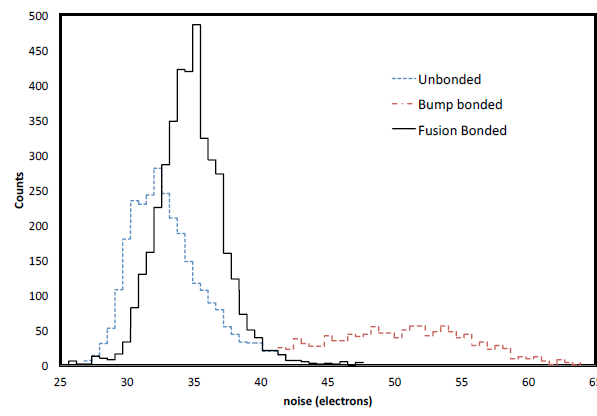
\includegraphics[width=0.45\textwidth]{fig_FastTiming/FusionBondedNoise.png}
        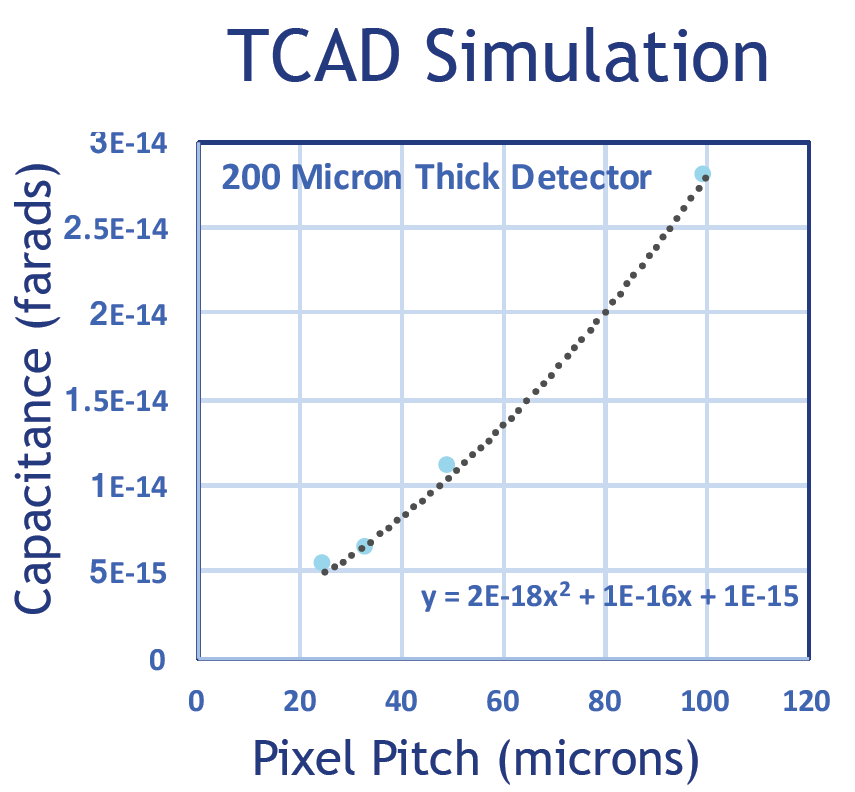
\includegraphics[width=0.35\textwidth]{fig_FastTiming/PixelPitch_Capacitance.png}
    \end{tabular}
    \caption{The noise in hybrid bonded VIPIC three-dimensional assembly is almost a factor of two lower than the equivalent conventionally bump bonded parts due to lower $C_L$ (Left).
            TCAD simulations predict that a smaller pixel pitch results in lower detector capacitance (Right).
            }            
    \label{FusionBondedNoise_PixelPitchCapacitance}
  \end{center}
\end{figure}
In general, 3DIC technologies have many potential implementations for integrating silicon sensors with dense readout electronics, with advantages including radiation hardness, low mass, and decreasing costs, that could make them ideally suited for application in high-energy particle silicon pixel detectors.

\section{Induced Currents for Fast Timing}
Signal current, as registered by an electrode, begins before any charge is collected by the electrode.  
Current is instantaneously induced in the electrode as electrostatic flux lines ending on the electrode change due to charges moving in the vicinity~\cite{doi:10.1063/1.1710367}.
According to the Ramo-Shockley theorem, current induced on an electrode in a multi-electrode system can be calculated from the coupling between the moving charge and the electrode, using a ``weighting field,'' depending on geometry and doping, that is determined by setting the potential of the electrode under consideration to unity, and setting the potential of all other electrodes to zero~\cite{1686997}.
The instantaneous current registered by an electrode by a charge moving in the vicinity can be expressed in terms of charge $q$, velocity $\vec{v}$, and weighting field $\vec{E_W}$ as:
\begin{linenomath*}
\begin{align}
i = -q \vec{v} \cdot \vec{E_W}
\end{align}
\end{linenomath*}
Induced currents have a very fast rise time, but if the charge is not collected by the electrode under consideration, then the induced signal current will change sign and integrate to zero.
For geometries where the pixel pitch is small compared to the substrate thickness, a charge moving far from the surface will induce currents in a cluster of electrodes surrounding the nodes that collect charge.
If detectors have sufficiently low capacitance and are integrated with fast electronics, the induced current signal can be utilized to provide timing information for four-dimensional tracking.

\section{FEA Simulations with TCAD}
Technology computer-aided design (TCAD) software is used to explore models for planar sensors in order to optimize the doping and geometry to achieve large induced currents with fast rise times.
The TCAD simulation uses finite element analysis (FEA) to simulate the electrical properties and behavior of semiconductor models, in this case by calculating the electric field in the model, the weighting fields of the individual electrodes, and the current induced at each electrode due to the motion of charge carriers in the substrate.
Both three-dimensional ($3 \times 3$) and two-dimensional ($1 \times 9$) models of pixel arrays, consisting of aluminum electrodes coupled to a silicon substrate, are simulated~\ref{Materials_Model}.
Different pixel pitches (\SI{25}{\micron} - \SI{100}{\micron}), substrate thicknesses (\SI{50}{\micron} - \SI{300}{\micron}), doping schemes ($n$-on-$n$, $n$-on-$p$), and bias voltages (\SI{100}{\V} - \SI{400}{\V}) were considered for these simulations.
Electrons are the preferred charge carrier, as they have higher mobility than holes and thus higher velocity, thereby inducing larger currents for the same electric field strength.
Even in the absence of an externally applied voltage, every $pn$-junction has a ``built-in'' electric field between the $p$ and $n$ sides from the thermal diffusion of mobile charge carriers.
For the doping scheme, $n$-on-$n$ has a maximal electric field near the bottom side, whereas $n$-on-$p$ has a maximal electric field near the top~\ref{Doping_ElectricField}.
Intermediate p-regions between electrodes, called ``$p$-stops,'' help shape the electric field and prevent unwanted diffusion of charges away from collecting electrodes.
\begin{figure}[htb]
  \begin{center}
    \begin{tabular}{cc}
      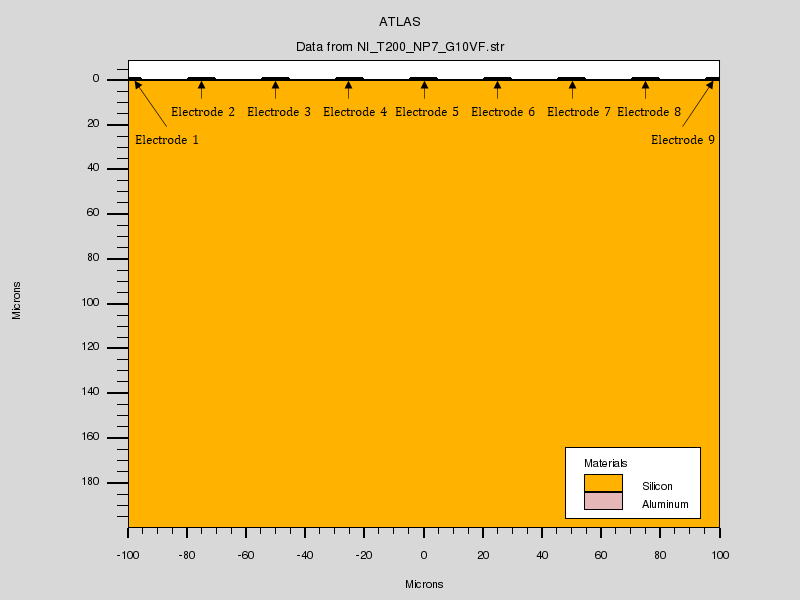
\includegraphics[width=0.45\textwidth]{fig_FastTiming/Materials.png}
      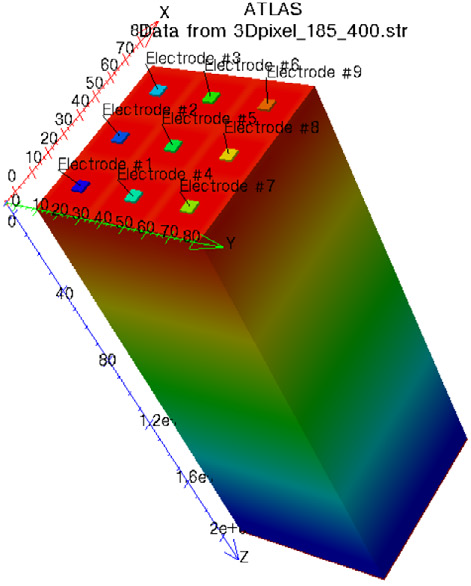
\includegraphics[width=0.275\textwidth]{fig_FastTiming/Model3D.png}
    \end{tabular}
    \caption{Two-dimensional $1 \times 9$ (Left) and three-dimensional $3 \times 3$ (Right) models of \SI{25}{\micron} pitch pixel arrays, consisting of aluminum electrodes (labeled) coupled to a silicon substrate.
            }
    \label{Materials_Model}
  \end{center}
\end{figure}
\begin{figure}[htb]
  \begin{center}
    \begin{tabular}{cc}
      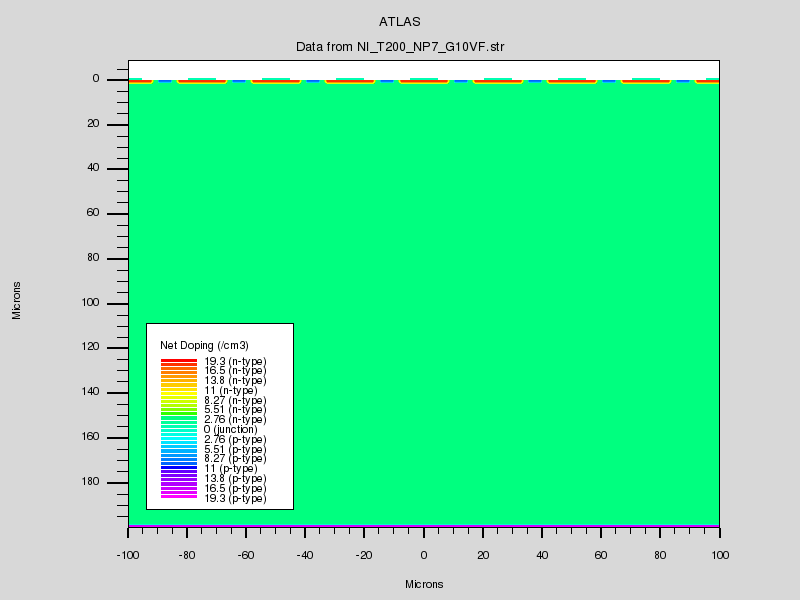
\includegraphics[width=0.45\textwidth]{fig_FastTiming/Net_Doping_nonn.png}
      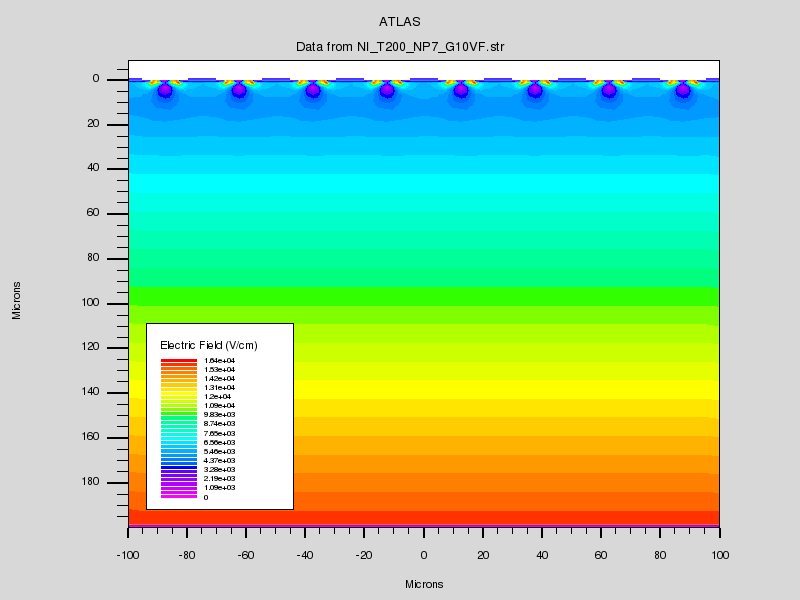
\includegraphics[width=0.45\textwidth]{fig_FastTiming/ElectricField_nonn.png} \\
      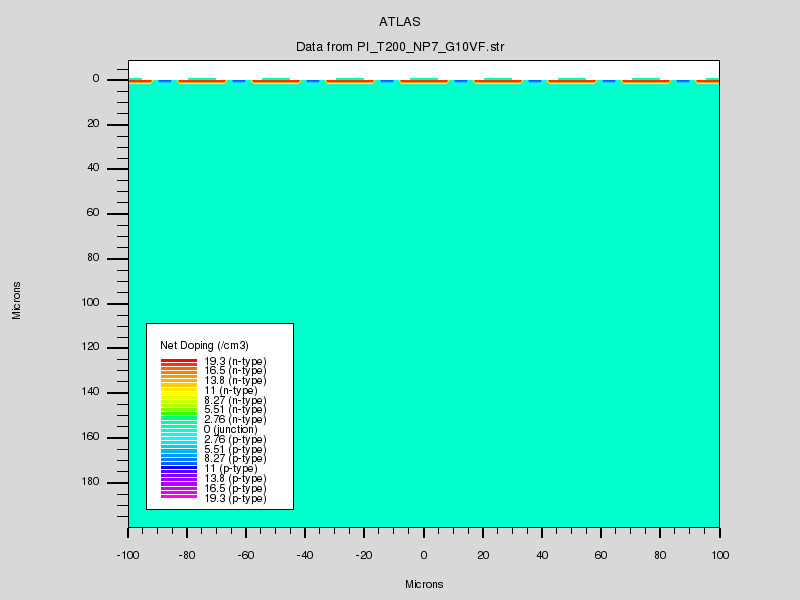
\includegraphics[width=0.45\textwidth]{fig_FastTiming/Net_Doping_nonp.png}
      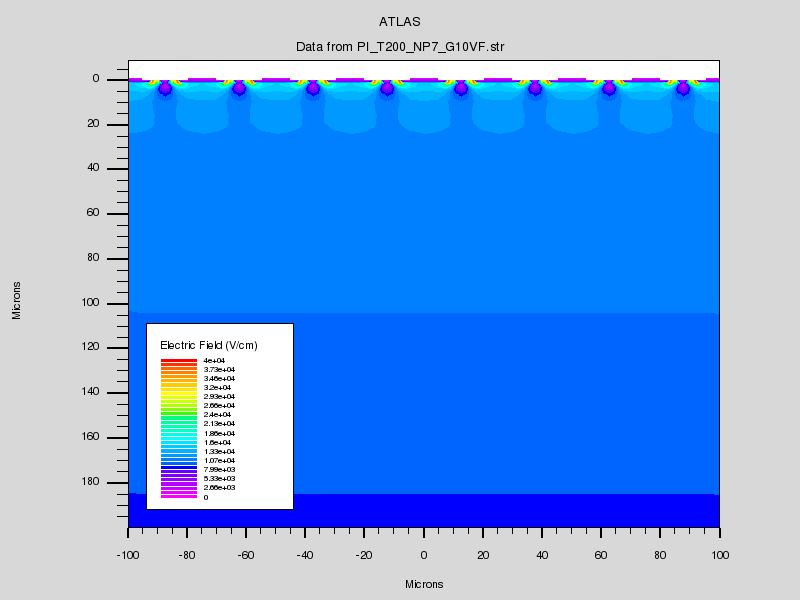
\includegraphics[width=0.45\textwidth]{fig_FastTiming/ElectricField_nonp.png} \\
    \end{tabular}
    \caption{Doping (Left) and built-in electric field (Right) profiles for TCAD simulated models of $1 \times 9$ (two-dimensional) array of pixels with 25 \si{\micron} pitch between aluminum electrodes coupled to a silicon substrate.
            $n$-on-$n$ (Top) has an electric field maximal near the bottom side, whereas $n$-on-$p$ (Bottom) has an electric field maximal near the top.
            }
    \label{Doping_ElectricField}
  \end{center}
\end{figure}

Two kinds of pulses were injected into the bulk of the substrate, either localized at a specific depth to simulate an absorbed x-ray, or uniformly through the depth at an angle of incidence to simulate ionization due to a MIP traversing the sensor.
Current density profiles visualizing the motion of mobile charges after ionization are shown in figures~\ref{CurrentDensity_xray} and~\ref{CurrentDensity_MIP} for an absorbed x-ray and MIP, respectively.
Simulated signal currents induced on electrodes by a locally ionizing x-ray at various depths and by uniformly ionizing MIPs at various angles of incidence are shown in figures~\ref{Signal_xray_Multi} and~\ref{Signal_MIP_Multi}, respectively.
The rich diversity of signal shapes in figure~\ref{Signal_MIP_Multi} demonstrates that thick detectors with small pixels have potential for distinguishing tracks as a function of the angle of incidence by using information from the collective pulse shapes of nearby pixels. 
The time between the initial current pulse and the peak current in a set of pixel shapes, for example, could be correlated in the readout electronics to measure the track angle.

\begin{figure}[htb]
  \begin{center}
    \begin{tabular}{c}
        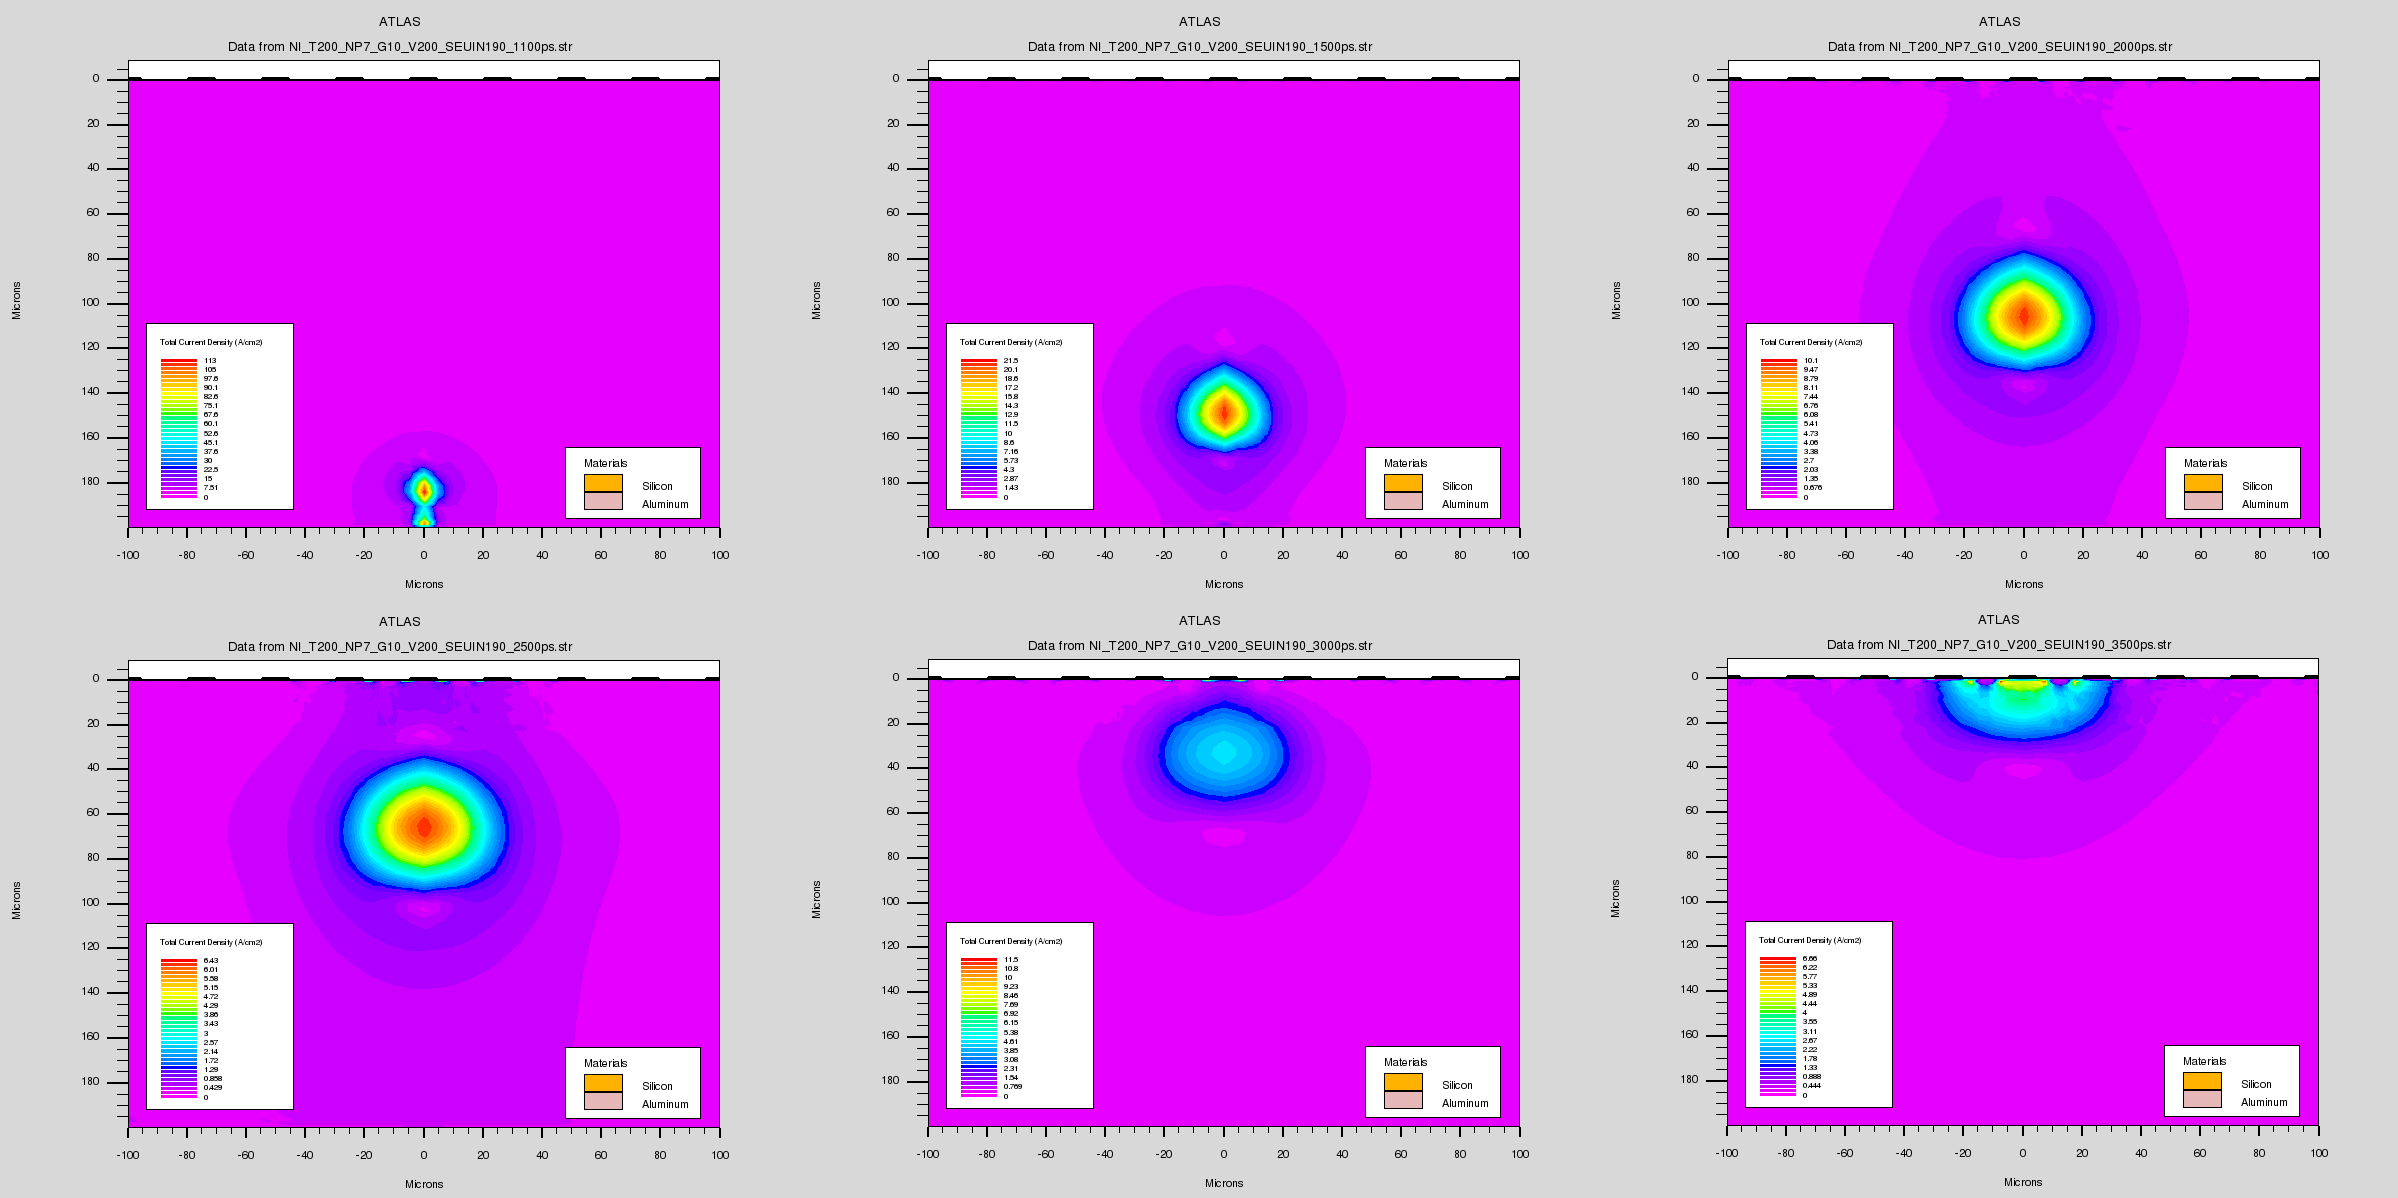
\includegraphics[width=.90\textwidth]{fig_FastTiming/CurrentDensity_xray.png}
    \end{tabular}
    \caption{Current density profiles visualizing the motion of mobile charges after localized ionization by an absorbed x-ray:
            .1 \si{\ns} (Top Left), .5 \si{\ns} (Top Middle), 1 \si{\ns} (Top Right), 1.5 \si{\ns} (Bottom Left), 2.0 \si{\ns} (Bottom Middle), 2.5 \si{\ns} (Bottom Right).
            The electrons drift upward towards the electrodes, and the holes drift downward.
            }
    \label{CurrentDensity_xray}
  \end{center}
\end{figure}
\begin{figure}[htb]
  \begin{center}
    \begin{tabular}{c}
        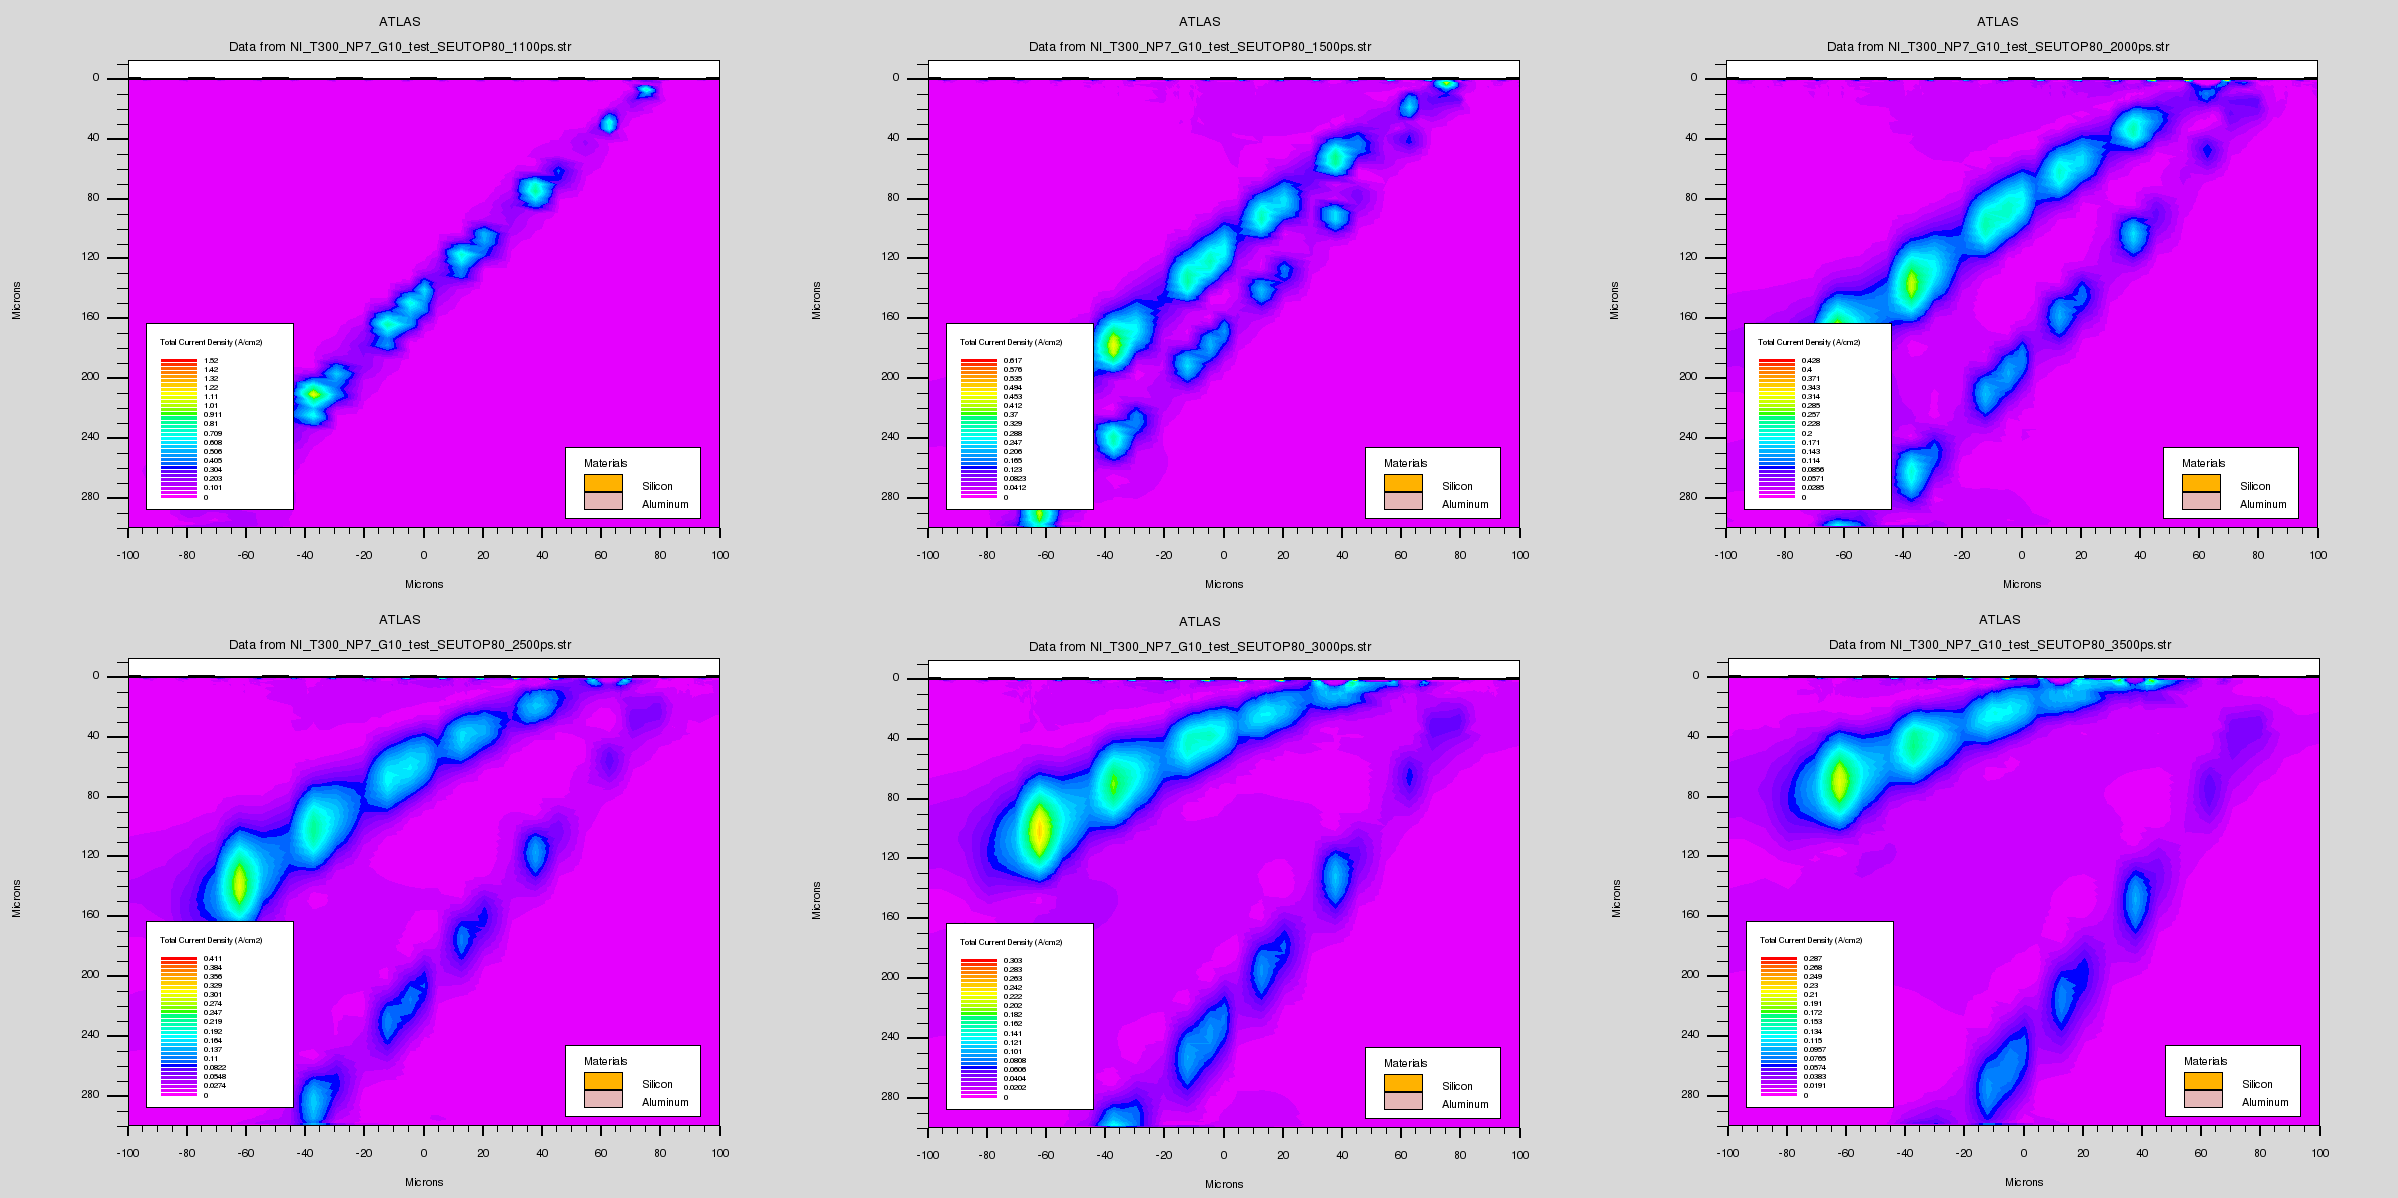
\includegraphics[width=.90\textwidth]{fig_FastTiming/CurrentDensity_MIP.png}
    \end{tabular}
    \caption{Current density profiles visualizing the motion of mobile charges after uniform ionization at an angle of incidence by a MIP:
            .1 \si{\ns} (Top Left), .5 \si{\ns} (Top Middle), 1 \si{\ns} (Top Right), 1.5 \si{\ns} (Bottom Left), 2.0 \si{\ns} (Bottom Middle), 2.5 \si{\ns} (Bottom Right).
            The electrons drift upward towards the electrodes, and the holes drift downward.
            }
    \label{CurrentDensity_MIP}
  \end{center}
\end{figure}

\begin{figure}[htb]
  \begin{center}
    \begin{tabular}{c}
        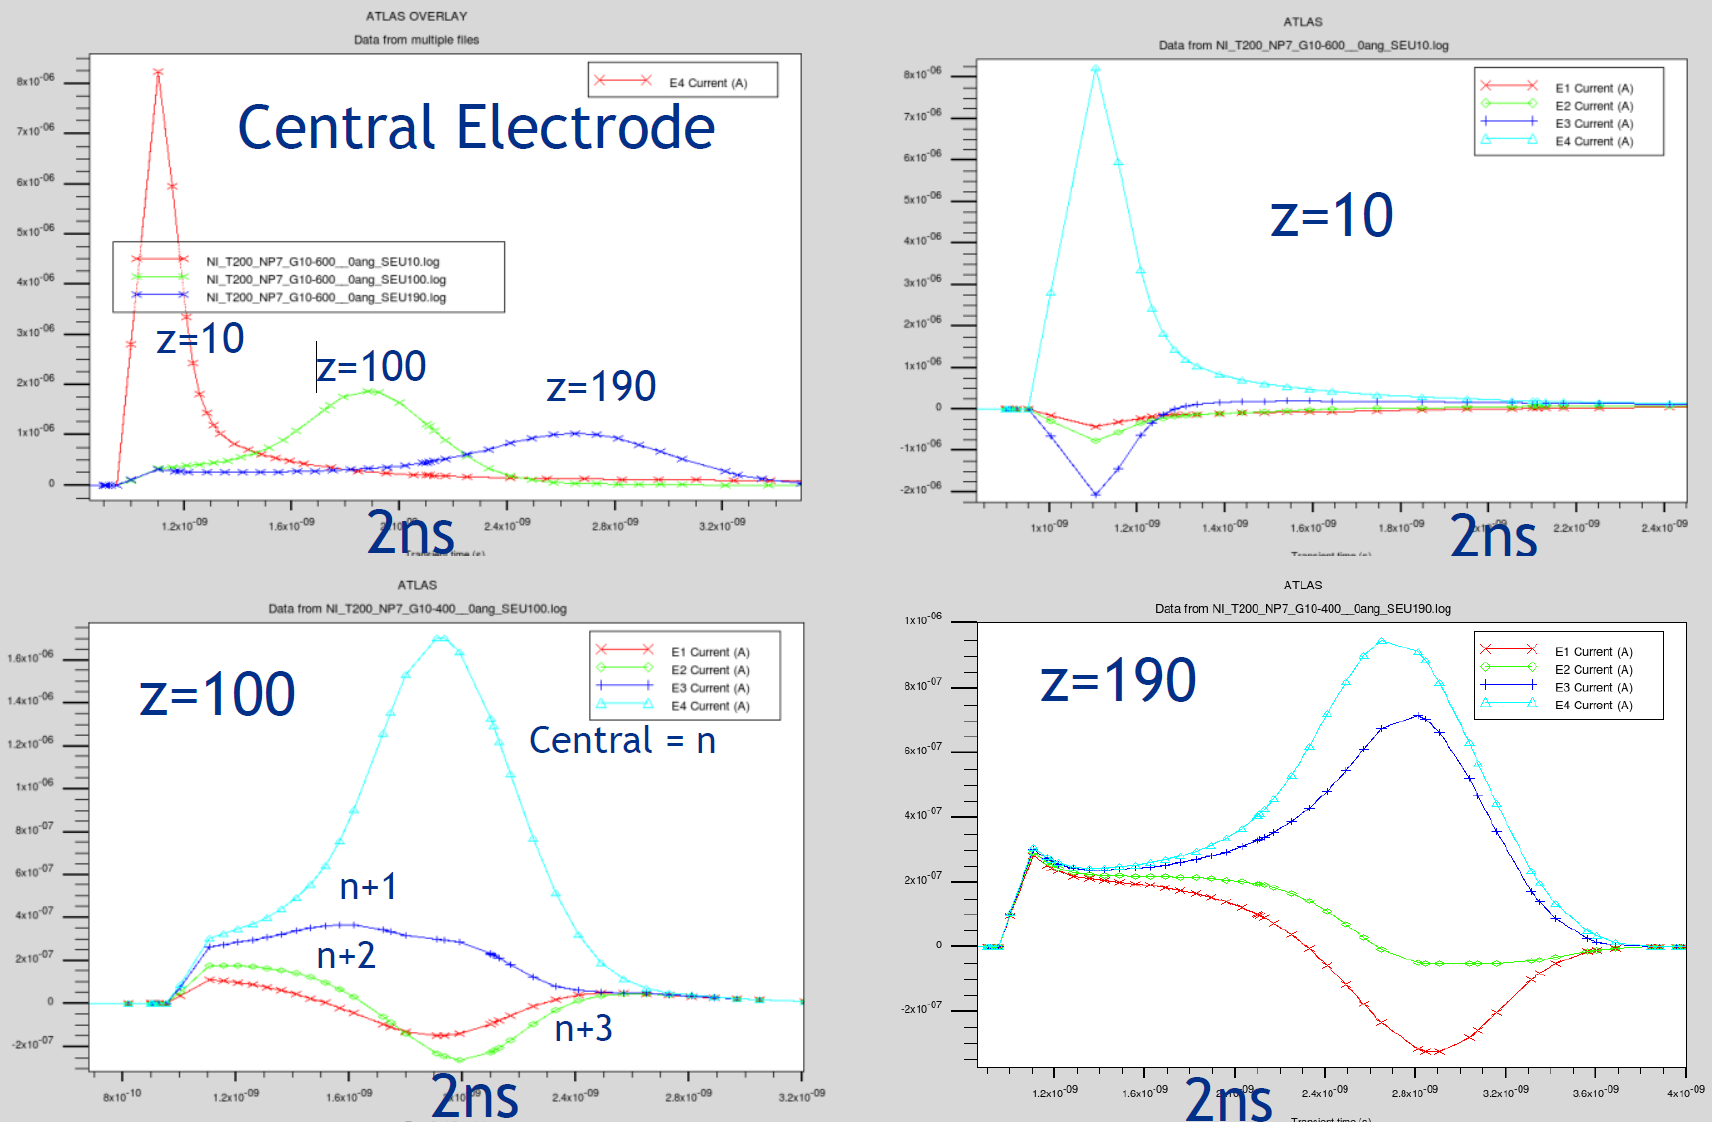
\includegraphics[width=.90\textwidth]{fig_FastTiming/Signal_xray_Multi.png}
    \end{tabular}
    \caption{Currents induced on electrodes by a locally ionizing x-ray at various depths (\SI{10}{\micron}, \SI{100}{\micron}, \SI{190}{\micron}) from the central electrode of a \SI{200}{\micron} thick detector with \SI{25}{\micron} pitch pixels biased at \SI{400}{\V}.
    The ionization is localized directly below Electrode 5 (E4).
            }
    \label{Signal_xray_Multi}
  \end{center}
\end{figure}
\begin{figure}[htb]
  \begin{center}
    \begin{tabular}{c}
        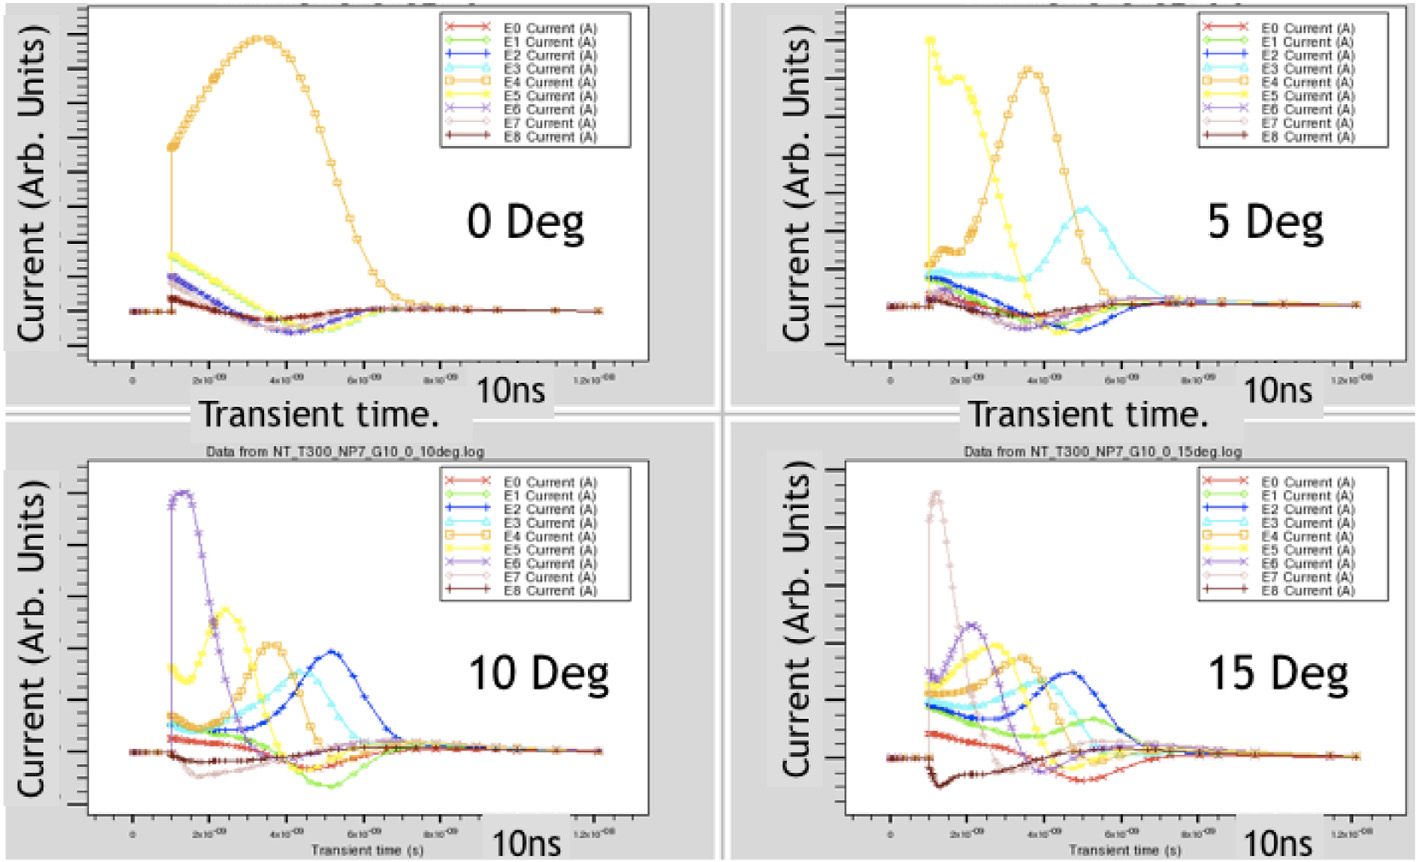
\includegraphics[width=.90\textwidth]{fig_FastTiming/Signal_MIP_Multi.png}
    \end{tabular}
    \caption{Currents induced on electrodes by a uniformly ionizing MIP at various angles of incidence with respect to the surface of a \SI{200}{\micron} thick detector with \SI{25}{\micron} pitch pixels biased at \SI{400}{\V}.
            The track at 0 degrees is incident on Electrode 5 (E4).
            }
    \label{Signal_MIP_Multi}
  \end{center}
\end{figure}

\section{Results}
The same pattern emerges that is most clearly demonstrated in the case of simulated x-ray absorption~\ref{Signal_xray}.
On the picosecond timescale, there is an initial current spike that is similar for all nearby pixels with a pitch small compared to ionization depth.
On the nanosecond timescale, charges-collecting electrodes detect a large signal current, but for electrodes not collecting charges, the current changes sign and integrates to zero.
\begin{figure}[htb]
  \begin{center}
    \begin{tabular}{c}
      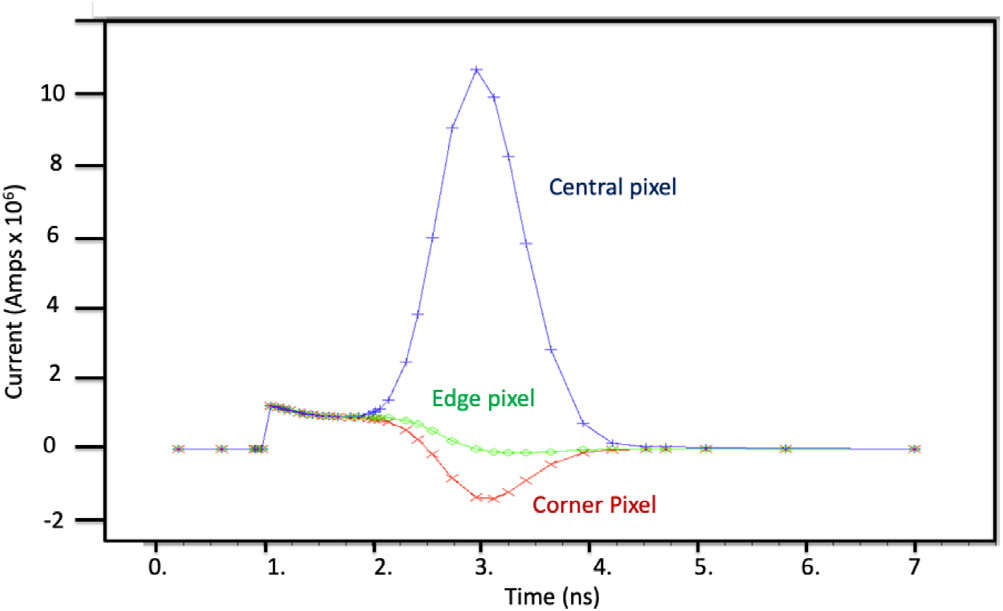
\includegraphics[width=0.50\textwidth]{fig_FastTiming/Signal_xray.png}
    \end{tabular}
    \caption{Signal for an X-ray deposited at \SI{190}{\micron} in a \SI{200}{\micron} thick detector with \SI{25}{\micron} pitch pixels biased at \SI{400}{\V}.
            }
    \label{Signal_xray}
  \end{center}
\end{figure}

The simulated currents are injected into a simulation program with integrated circuit emphasis (SPICE) model of a \SI{65}{\nm} technology amplifier, including noise, and current supplied to the input transistor around 4 $\mu A$.
The pulse shape from the central electrode peaks at \sim$\SI{1}{\V}$ after \sim$\SI{12}{\ns}$, and the edge electrode peaks at \sim$\SI{25}{\mV}$ after \sim$\SI{2}{\ns}$.
The threshold is set at \SI{130}{\mV} above baseline for the central electrode and \SI{10}{\mV} above baseline for the edge electrode.
The jitter timing resolution is extracted from a Gaussian fit of the arrival times of an ensemble of resulting pulses that differ only due to jitter noise.
\begin{figure}[htb]
  \begin{center}
    \begin{tabular}{c}
      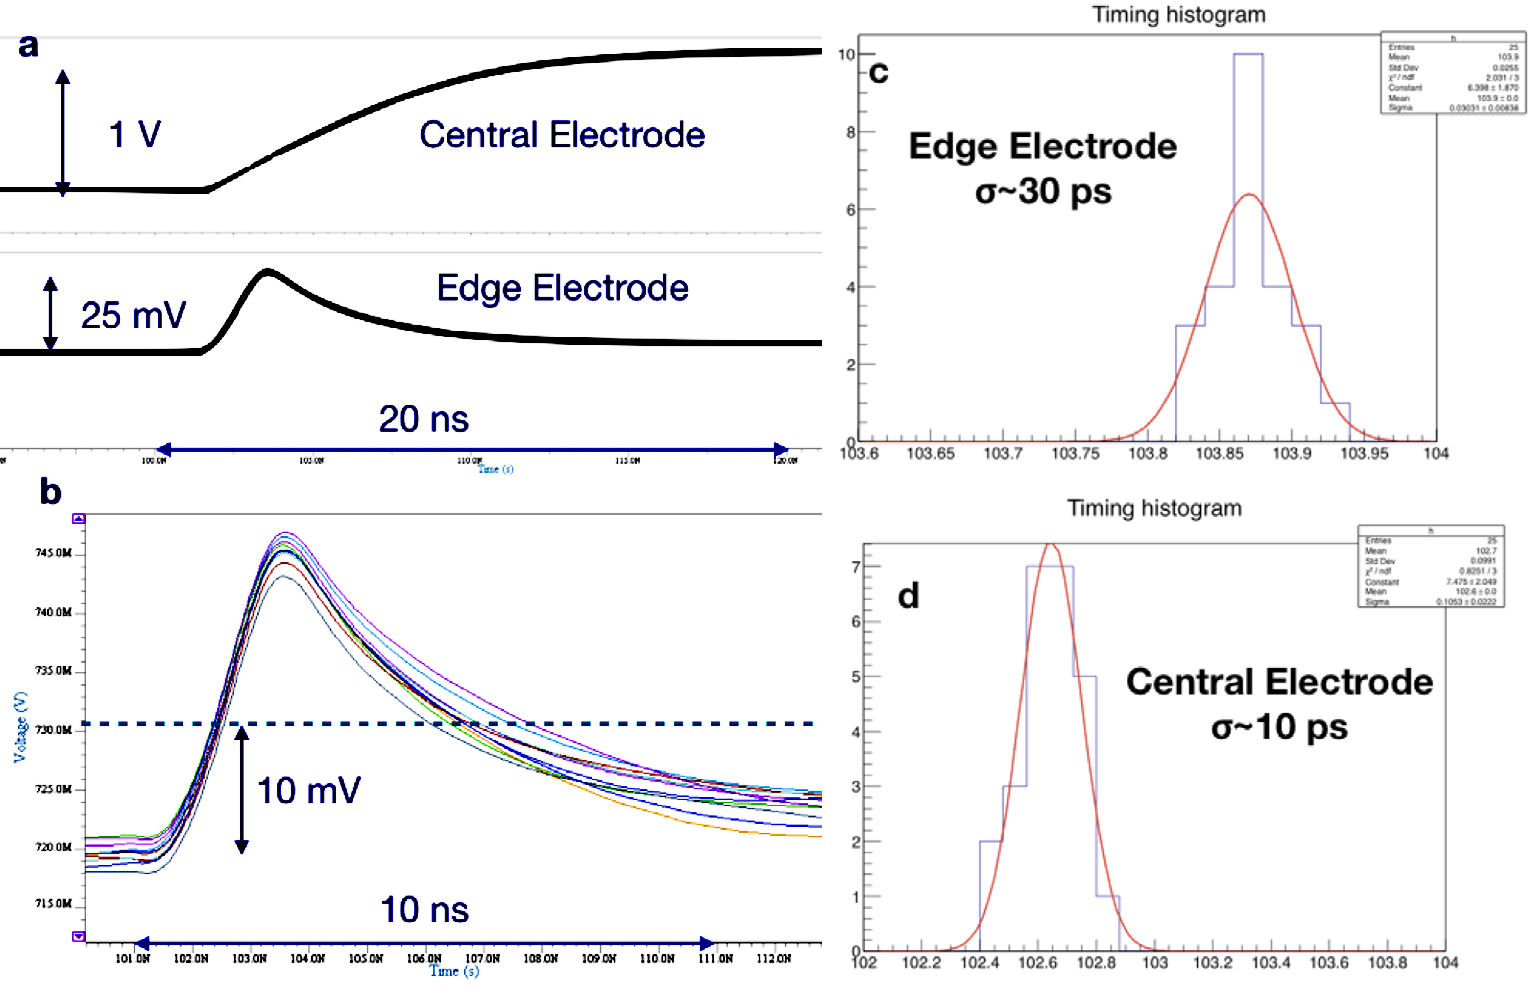
\includegraphics[width=0.80\textwidth]{fig_FastTiming/TimingResolutions.png}
    \end{tabular}
    \caption{Pulse shapes and jitter timing resolution, of central (charge collecting) and edge (induced current) electrodes, for a simulated x-ray ionization at a depth of \SI{185}{\micron} in a \SI{200}{\micron} thick detector.
        (a) Pulse shapes for the central and edge electrode. 
        (b) Pulse shape for the edge electrode for 25 pulses, including noise, with the threshold set at \SI{10}{\mV} above baseline.
        (c) The jitter timing resolution for the edge electrode in plot b.
        (d) The jitter timing resolution for the central electrode with a threshold of \SI{130}{\mV} above the baseline.
            }
    \label{TimingResolutions}
  \end{center}
\end{figure}

The resulting jitter time resolution~\ref{TimingResolutions} is \sim$\SI{10}{\ps}$ for central electrodes and \sim$\SI{30}{\ps}$ for edge electrodes, which indicates that noise-induced jitter will likely not be a dominant factor for timing resolution with small pixels.
Time walk and ionization fluctuation components of timing resolution were not considered in this limited study.

As a concluding remark, small pixel detector systems show promise for addressing some of the extreme challenges of future high-energy particle experiments, including precise position and timing resolution, complex event topology, and radiation hardness.
This study considers some toy models, but for real application of these ideas, there are many more electronics and system engineering considerations that need to be studied.